\documentclass{scrartcl}

%% Language and font encodings
\usepackage[english]{babel}
\usepackage[utf8x]{inputenc}
\usepackage[T1]{fontenc}

%% Sets page size and margins
\usepackage[a4paper,top=3cm,bottom=2cm,left=3cm,right=3cm,marginparwidth=1.75cm]{geometry}

%% Useful packages
\usepackage{amsmath}
\usepackage{graphicx}
\usepackage[colorinlistoftodos]{todonotes}
\usepackage[colorlinks=true, allcolors=blue]{hyperref}

%% bibliography
\usepackage[square,numbers]{natbib}
\bibliographystyle{abbrvnat}
\title{Discrete event simulation of different selfish mining strategies in Bitcoin}
\subtitle{Master Thesis Proposal}
\author{Advisor: Edgar Weippl}

\begin{document}
\maketitle

\section{Problem statement}
The cryptocurrency Bitcoin started back in the year 2008 with the release of the Bitcoin white paper \cite{nakamoto2008bitcoin} and reached as of today a market capitalization of over 20 billion dollars \cite{MarketCap2017, Coindesk2017}. Internally the Bitcoin cryptocurrency records all transactions in a public ledger called the blockchain. The blockchain is basically an immutable linked list of blocks where a block contains multiple transactions of the cryptocurrency. In Bitcoin, each block needs to contain a so-called proof of work (PoW) which is the solution to a costly and time-consuming cryptographic puzzle. Miners connected in a peer-to-peer network compete with their computation power to find solutions to the puzzle and hence to find the next block for the blockchain. Finding a block allows the miners to add a transaction to the block and gives them a certain amount of bitcoins out of thin air. Additionally, the grouping of the transaction in blocks creates an ordering for the transaction and makes it possible to prevent double-spending. After a block is found by a miner all other miners should adopt to this new tip of the chain and try to find a new block on top. This mining process is considered as incentive compatible as long as no single miner has more than 50\% of the total computation power.

\citeauthor{eyal2014majority} showed that also miners under 50\% have an incentive to not follow the protocol as described depending on their connectivity in the peer-to-peer network and computation power. By implementing a so-called selfish mining strategy a miner can obtain relatively more revenue than his actual proportion of computational power in the network. In general, the miner simply does not shares found blocks with the others and secretly mines on his own chain. At some point, the public miners will catch up with their public chain because they have over 50\% of the computation power. In this case, the selfish miner publishes his blocks. If his chain is longer then the public chain, he is able to overwrite all blocks found by the honest miners. If the two chains have the same length the private miner also publishes his block and causes a block race. Now the network is split into two parts where one part is mining on the public tip and the other part is mining on the now public-private tip. In general, the selfish miner achieves that the other miners are wasting their computational power on blocks which will not end up in the longest chain.

%Nevertheless, in the short run, the selfish mining is not always profitable. Because of the waste of computational power caused by selfish mining fewer blocks are found. The selfish miner can increase his relative share but since there are fewer blocks often the honest behaviour would be more profitable. The selfish miner has to wait until the difficulty of the PoW-puzzle is adjusted to the now lower computational power of the network which happens in Bitcoin every two weeks. \cite{gervais2016security, nayak2016stubborn}

Further research \cite{nayak2016stubborn,sapirshtein2016optimal, gervais2015tampering, gervais2016security, bahack2013theoretical} explored different modifications of the original selfish mining algorithm by \citeauthor{eyal2014majority} and found slightly modifications of the algorithm which perform better under certain circumstances. For example, it could make sense for the selfish miner to even trail behind the public chain.

To prove the existence and attributes of selfish mining different approaches were applied. The researchers used simple probabilistic arguments \cite{eyal2014majority, bahack2013theoretical}, numeric simulation of paths with state machines \cite{gervais2015tampering, nayak2016stubborn}, advanced Markov Decision Processes (MDP) \cite{sapirshtein2016optimal, gervais2016security} or gave results of closed-source simulations \cite{eyal2014majority, sapirshtein2016optimal}. Unfortunately, we cannot discuss the closed source simulations but all other methodologies do not use discrete event simulation (DES) \cite{fishman1978principles} to simulate selfish mining. This type of simulation would allow reducing the abstraction used in the above-mentioned methodologies. One of the main abstraction introduced by the other researchers is that they model the block races with a simple probabilistic distribution. With a DES-simulation, it would be possible to model the whole network topology and simulate selfish mining under more realistic conditions. Hence the simulation could capture network delays and natural forks of the chain.

\section{Expected result}
The expected outcome of this thesis is a DES-simulation of different selfish mining strategies. The selfish mining strategies include:
\begin{itemize}
\item selfish mining \cite{eyal2014majority}
\item lead stubborn mining \cite{nayak2016stubborn}
\item trail stubborn mining \cite{nayak2016stubborn}
\item equal-fork stubborn mining \cite{nayak2016stubborn}
\end{itemize}

For the simulation these strategies are combined with different distributions of computation power between the nodes and different network topologies. The result of the simulations should show which strategy is the best strategy for a certain combination of a network topology and distribution of computation power. 

Furthermore, the simulations should emphasise the recent work in the area of selfish mining and show that the current implementation of Bitcoin protocol is vulnerable against different selfish mining strategies.

\section{Methodology and approach}
First, the different mining strategies selfish, lead stubborn, trail stubborn and equal-fork stubborn mining from \citeauthor{nayak2016stubborn} and \citeauthor{eyal2014majority} need to be implemented. This is achieved by implementing a proxy which eclipses a normal Bitcoin client from the other nodes in the network. Now, if a block is found the proxy decides, depending on his selfish mining strategy, if a block should be transmitted from the eclipsed node to the rest of the network or vice versa. The design pattern proxy makes it possible to implement the selfish mining strategies without altering the reference implementation of Bitcoin and is therefore preferred over an implementation directly in the Bitcoin client.

In the next step, a DES-simulation program is implemented. To be able to control when a certain node finds a block all Bitcoin nodes are executed in test mode. In test mode the real proof of work algorithm is disabled and every node accepts a command which lets the node create immediately a new block. With this functionality, it is possible to define a block discovery series which basically reflects the computation power of each node. The more blocks are found by a node the more simulated computation power the node has. Additionally to the block generation, the simulation program should also control the network topology and hence the connectivity of each node. For the simulation run, it is important that the connectivity of the nodes stays the same to make the results better comparable. This should be achieved by setting the connections from the nodes by the simulation program itself which is in contrast to normal behaviour. Normally Bitcoin nodes share their connections with other nodes over the Bitcoin protocol and try to improve the connectivity over time.

After the implementation of the selfish mining strategies and the DES-simulation program, the mining strategies are simulated. Different settings for the connectivity and distribution of computation power are used to compare the profitability of the selfish mining strategies to the normal, honest mining.

\section{State-of-the-art}
Already in the year 2010 the user \textit{ByteCoin} described the idea of selfish mining in the Bitcoin forum \textit{bitcointalk} \cite{ByteCoin2010}. He provided simulation results of the attack which at that time was called \textit{mining cartel attack}. Nevertheless, the discussions in the thread never caught fire and no further investigations or countermeasures were taken by the community \citep{BitcoinTalk2010, bahack2013theoretical}.

Later in 2014 \citeauthor{eyal2014majority} released the paper \textit{"Majority is not enough: Bitcoin mining is vulnerable."} and coined the term selfish mining. The paper gives a formal description of selfish mining and proves how a miner can earn more than his fair share by conducting the attack. Figure \ref{fig:selfish_mining} shows the attack as a state machine where $\alpha$ denotes the mining power share of the selfish miner. The labels of the states are representing the lead of the selfish miner over the public chain. The state \textit{0'} shows a possible block race between the public block and the released private block. In the case of a block race, the variable $\gamma$ denotes the probability of the selfish miner to win the block race. Hence $\gamma$ part of the miners are mining on the public-private block and respectively (1 − $\gamma$) are mining on the public block. The labels on the transitions are representing the transition probabilities between the states. The profitability of the simple strategy was proved by applying probability calculations. Furthermore, results of an undisclosed Bitcoin protocol simulator were given. In the simulation, 1000 miners with the same simulated mining power were simulated and a fraction of these miners formed a pool which applied the selfish mining algorithm. In the case of a block race they artificially split the network where one part is mining on the public block and one part is mining on the block of the selfish pool.


\begin{figure}[t]
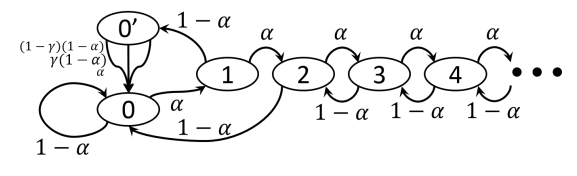
\includegraphics[width=8cm]{figures/selfish_mining}
\centering
\caption{Selfish mining state machine with transition probabilities \cite{eyal2014majority}}
\label{fig:selfish_mining}
\end{figure}


Further research showed that more generalised selfish mining strategies lead to even more relative gain for the selfish miner \cite{nayak2016stubborn,sapirshtein2016optimal, gervais2015tampering, gervais2016security, bahack2013theoretical}. Figure \ref{fig:stubborn_mining} shows a possible categorization of the different selfish mining strategies where $\alpha$ and $\gamma$ is used equivalent as in figure \ref{fig:selfish_mining} and $\beta$ = (1 − $\alpha$). Furthermore, the prime states are denoting states where a block race happens on certain height and the state \textit{0''} represent the state where both chains have the same height but with a different tip. The idea behind the different variations of selfish mining in figure \ref{fig:stubborn_mining} are:
\begin{itemize}
\item Lead stubborn mining strategy compromises the idea to cause as many block races as possible and to never overwrite the public chain with a longer chain. This strategy is especially promising when the probability to win the block race is very high.
\item Equal-fork stubborn mining strategy changes the selfish mining strategy just by one transition. In case the selfish miner wins a block race, he does not publish his block to win the race but he also keeps this block undisclosed to have an advantage over the other miners.
\item Trail stubborn mining strategies reflects the idea to even trail behind the public chain and to eventually catch up. The figure \ref{fig:stubborn_mining} depicts the trail stubborn mining strategy \textit{T1}. The number one denotes that the selfish miner is allowed to trail one block behind the public chain.
\end{itemize}

The strategy space for a selfish miner is practically endless and combinations of the aforementioned strategies are possible and are leading to even more relative gain. \cite{nayak2016stubborn,sapirshtein2016optimal, gervais2015tampering, gervais2016security, bahack2013theoretical}


\begin{figure}[t]
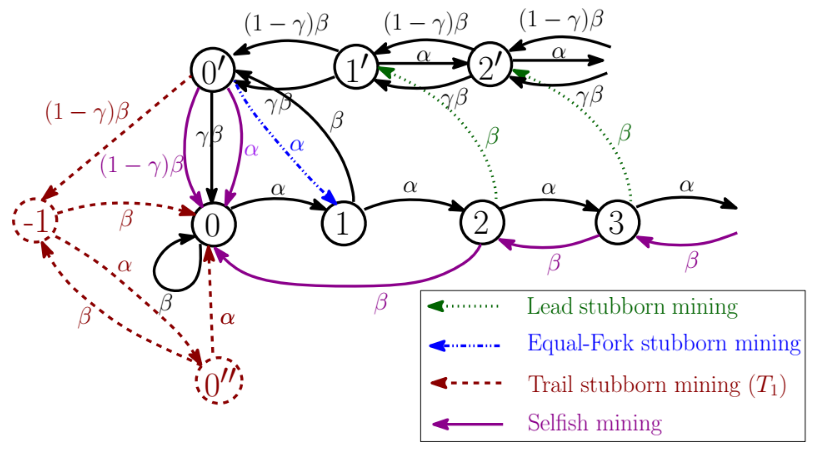
\includegraphics[width=10cm]{figures/stubborn_mining}
\centering
\caption{Categorization of different mining strategies \cite{nayak2016stubborn}}
\label{fig:stubborn_mining}
\end{figure}


To find the best strategy for a given mining power share $\alpha$ and connectivity $\gamma$ researchers used two methodologies. \cite{gervais2015tampering, nayak2016stubborn} used numeric simulations based on a state machine to find optimal selfish mining strategies. \cite{sapirshtein2016optimal, gervais2016security} on the other hand used MDPs based on a state machine to find strategies with the most relative gain. The basic principle of the used state machines is for all publications the same. To validate their results \citep{eyal2014majority, sapirshtein2016optimal} additionally used a closed-source simulation.

Besides using variations of the selfish mining strategies, the attack can also be combined with other attacks to achieve better results \cite{gervais2016security, sapirshtein2016optimal, nayak2016stubborn, gervais2015tampering}. If the eclipse attack is used in combination with selfish mining the victim contributes its mining power to the private chain and hence, strengthens the position of the selfish miner \cite{nayak2016stubborn, gervais2016security}. \cite{nayak2016stubborn} additionally shows that the eclipsed victim under certain circumstances can benefit from the attack and therefore has no incentive to stop the attack. Another attack which can be used in combination with selfish mining is double-spending \cite{sapirshtein2016optimal, gervais2016security}. Every time the selfish miner starts his selfish mining attack he can publish a transaction and include a conflicting transaction in his first secret block. During the execution of the selfish mining attack, the payment receiver may accept the payment depending on his block confirmation time. Now in the case of a successful selfish mining attempt, the adversary can overwrite the public chain, which additionally results in a successful double spending. The operational costs of unsuccessful double-spending can be seen as low because the adversary still would get some goods in exchange for the transaction \cite{sapirshtein2016optimal, gervais2016security}.

Last but not least also the prevention of selfish mining is part of the current work in research\cite{eyal2014majority, billah2015one, solat2016zeroblock, zhang2017publish}. A backwards-compatible patch to mitigate selfish mining is uniform tie-breaking \cite{eyal2014majority}. This means whenever a node receives two blocks of the same height he randomly select on of the blocks to mine on. \citep{eyal2014majority} showed that this would raise the profit threshold to 25\% of the computational power. Later \citep{sapirshtein2016optimal} showed that the threshold would be only 23.21\%. Furthermore, the change would raise the connectivity of badly connected miners to almost 50\% with no actual effort for the attacker. Another countermeasure foresees unforgeable timestamps to secure Bitcoin against selfish mining \citep{billah2015one}. This countermeasure would make all pre-mined blocks of the selfish miner invalid after a certain amount of time. The drawback is the additional time-stamping functionality with random beacons \citep{billah2015one}. \cite{zhang2017publish} proposes backward-compatible countermeasure by neglecting blocks that are not published in time and allows incorporation of competing blocks in the chain similar to Ethereum's uncle blocks \cite{Ethereum}. This enables a new fork-resolving policy where a block always contributes to neither or both branches of the fork \cite{zhang2017publish}.

\section{Relation to "Software Engineering and Internet Computing" curriculum}
Bitcoin, the overlying topic, is a relatively new technology. Hence there are no concrete subjects or modules teaching this technology in the current curriculum. But under the hood Bitcoin technically is just a composition of different technologies which can be related to modules of the curriculum. First of all, Bitcoin is a software acting as a distributed system and can, therefore, be linked to the modules \textit{Software Engineering} and \textit{Distributed Systems}. Furthermore, Bitcoin uses cryptography to secure the system, which can be linked to the module \textit{Advanced Security}. Hash functions are the main component of the PoW-algorithm in the mining process which helps to prevent double spending. Furthermore digital signatures based on cryptography are used to secure the bitcoins held by the different users of the system.

In the thesis, the implementation of a proxy enabling selfish mining strategies and a DES-simulation program are carried out. Since both of them are an implementation effort they can be directly linked to the module \textit{Software Engineering}. Furthermore, both software programs are related directly to the module \textit{Distributed Systems}. The proxy needs to be suited between multiple nodes in a Bitcoin network which is a distributed system and the simulation program needs to start-up, manage and tear-down this distributed system.

\bibliography{sample}

\end{document}